After primary experiments on toy examples, we wanted to asses the effectiveness of GOAT in detecting bugs.
%
We evaluated GoBench

68 bugs

Built-in deadlock detector misses some bugs
Lock-based deadlock detectors misses some bugs
GoLeak misses some
Goat misses some

\subsubsection{GoBench}
\label{sec:gobench}
\begin{itemize}
  \item Introduce GoBench
  \item GoKer (68 blocking + 35 non-blocking (race)) TOT=103
\end{itemize}
\subsubsection{Results}
\label{sec:results}

\subsubsection{Discussion}
\label{discussion}


\begin{figure}
\centering
  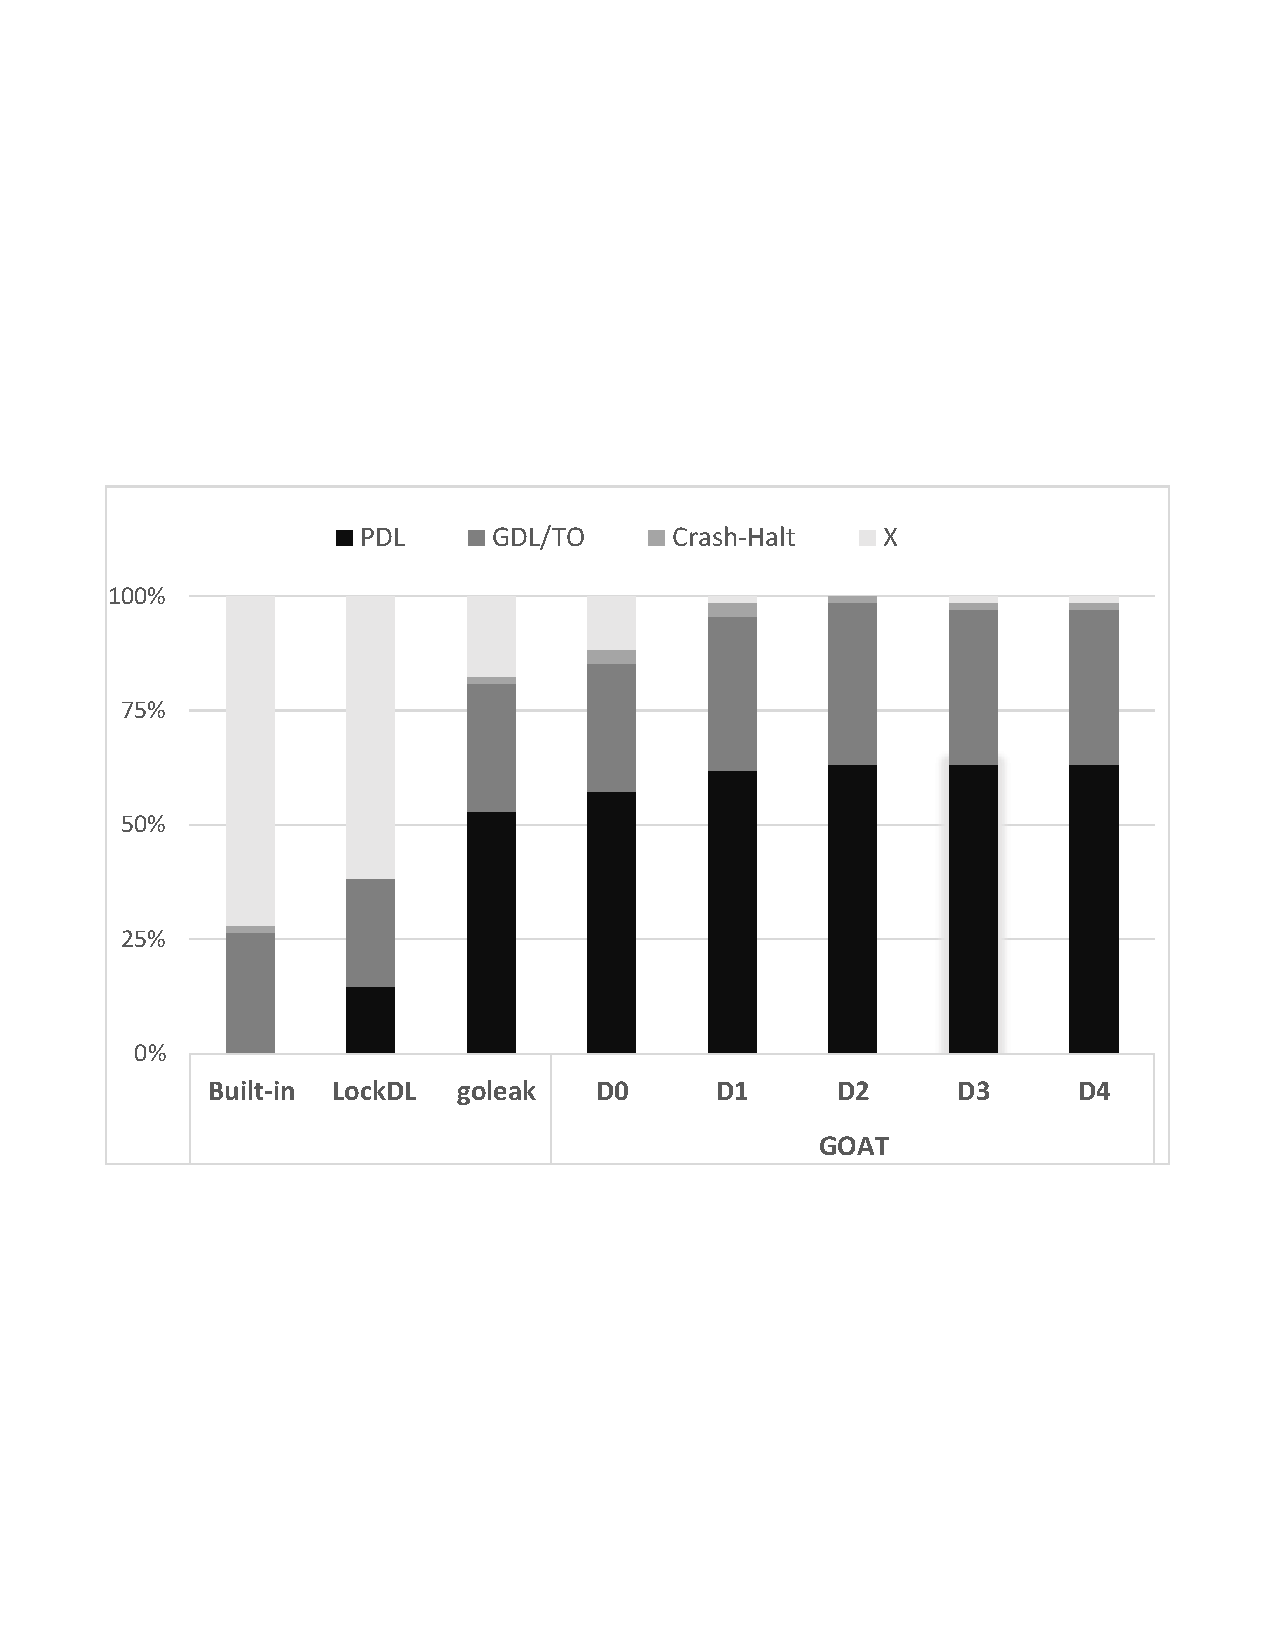
\includegraphics[width=.95\linewidth]{figs/P4_detections.pdf}
  \caption{Distribution of detected bugs by built-in deadlock detector (BUILTINDL), LockDL, GoLeak, and GOAT different d. (over 1000 runs). pdl: partial deadlock, gdl: global deadlock, crash/halt: causes the program to crash or halt on detection, x: nothing is detected }
  \label{fig:detection}
\end{figure}


\begin{figure}
\centering
  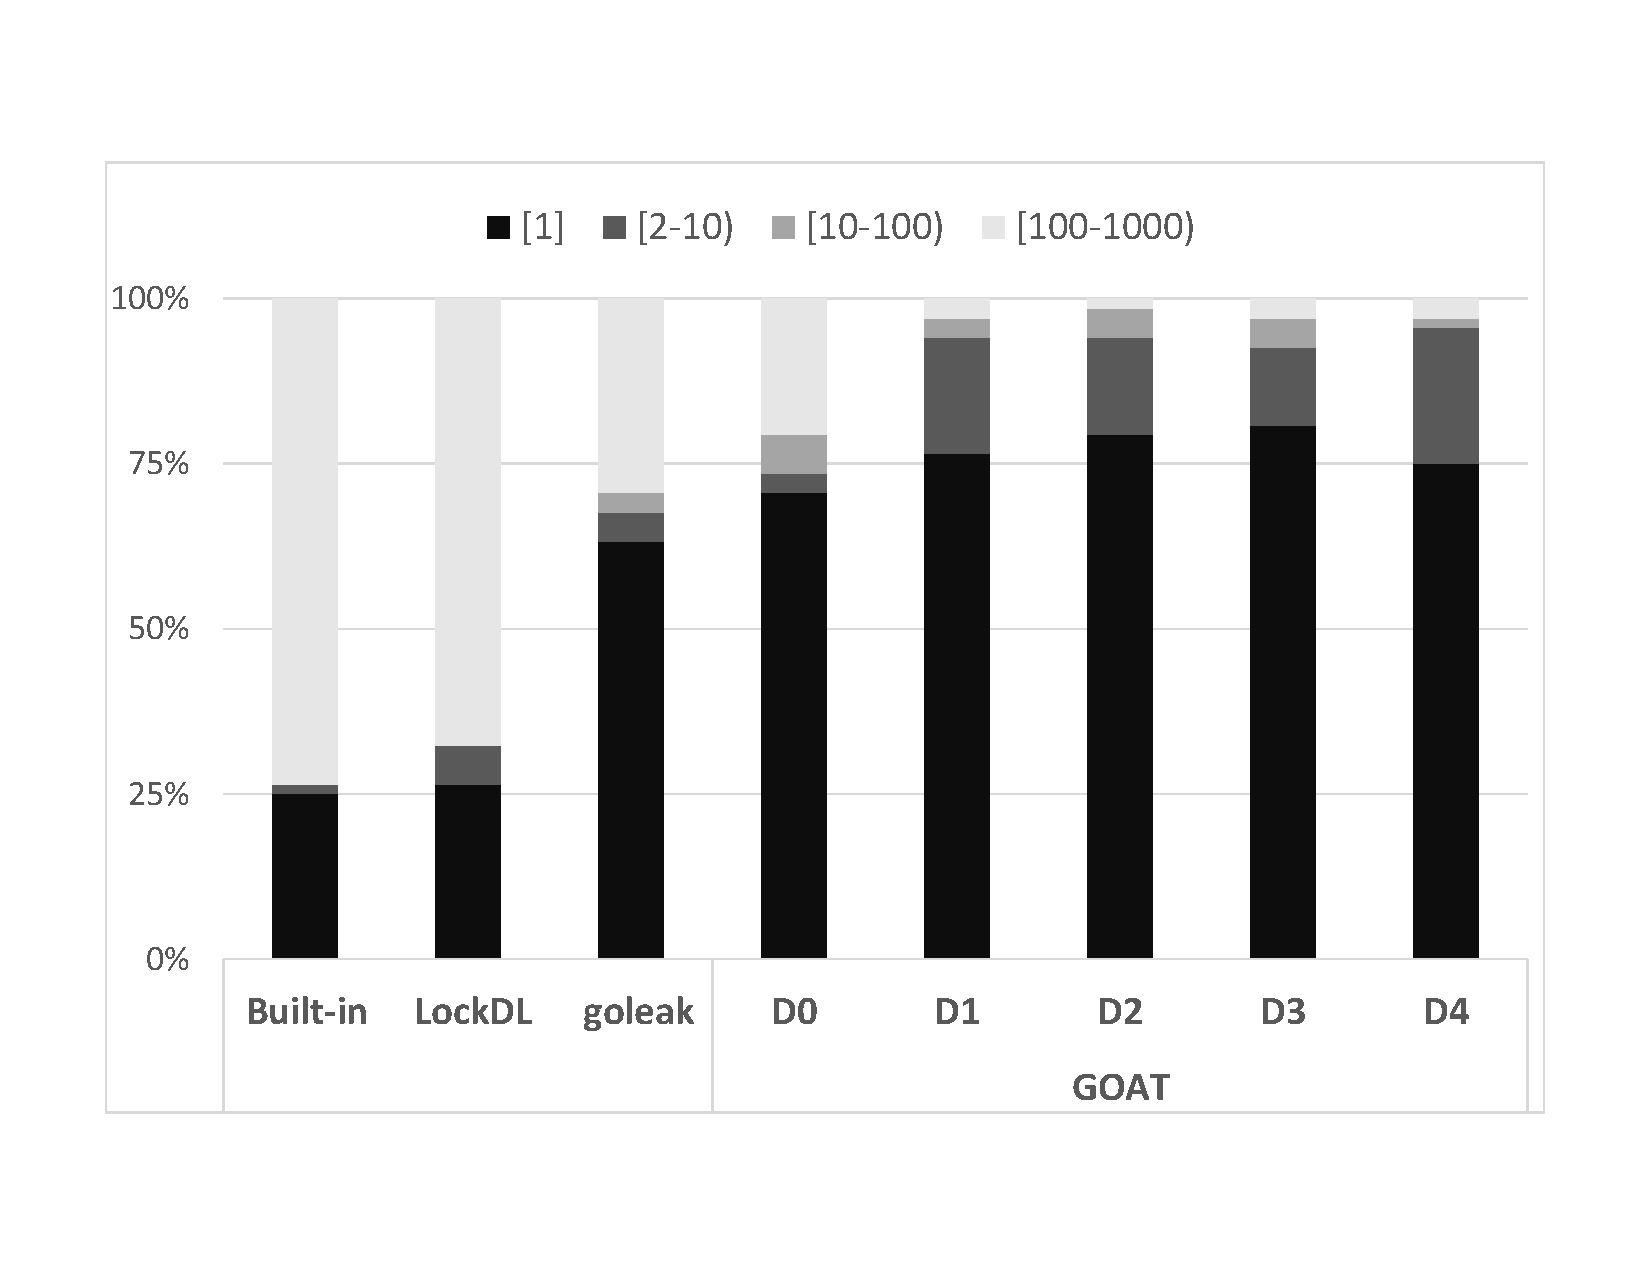
\includegraphics[width=.95\linewidth]{figs/P4_runs.pdf}
  \caption{Distribution of required number of iterations to detect the bug for each tool}
  \label{fig:runs}
\end{figure}
